\subsection{Some Standard Mappings of the Plane}

\begin{tcolorbox}[title=Problem 1, breakable]
    Let $F$ be a mapping of the plane into itself.
    We define a \textbf{fixed point} for $F$ to be a 
        point $P$ such that $F(P) = P$. \\

    Describe the fixed points of the following mappings.

    (a) The identity.

    (b) Reflection through a given point $O$.

    (c) Reflection through a line.

    (d) A rotation not equal to the identity, with respect to a given point $O$.

    (e) A translation not equal to the identity.

    (f) Dilation by a number $r > 0$, relative to a given point $O$.
\end{tcolorbox}

\textbf{Solution (a):}

All points in the plane are fixed points.

\textbf{Solution (b):}

The point $O$ is a fixed point.

\textbf{Solution (c):}

All points on the line are fixed points.

\textbf{Solution (d):}

The point $O$ is a fixed point.

\textbf{Solution (e):}

There are no fixed points on the plane.

\textbf{Solution (f):}

If $r = 1$, then all points are fixed points.  
If $r \neq 1$, then only $O$ is a fixed point.

\subsection{Isometries}

\begin{tcolorbox}[title=Problem 2, breakable]
    For which values of $r$ is dilation by $r$ an isometry?
\end{tcolorbox}

When $r = 1$ or $r = -1$.

\begin{tcolorbox}[title=Problem 4, breakable]
    Let $L, K$ be two parallel lines, and let $F$ be an isometry.
    Prove that $F(L)$ and $F(K)$ are parallel.
\end{tcolorbox}

\begin{proof}
    If $L = K$ then trivially $F(L)$ and $F(K)$ are parallel as they are equal
        since $F$ is an isometry.

    Suppose $L \not = K$.
    For contradiction, suppose $F(L)$ and $F(K)$ are not parallel.
    Then there is a point where $F(L)$ and $F(K)$ intersect.
    Since $F$ is an isometry, this would imply that $L$ and $K$ also intersect,
        contradicting the fact that $L$ and $K$ are distinct parallel lines.
\end{proof}

\begin{tcolorbox}[title=Problem 5, breakable]
    Let $K, L$ be perpendicular lines, and let $F$ be an isometry.
    Prove that $F(K)$ and $F(L)$ are perpendicular. [Hint: Use the 
    corollary of the Pythagoras theorem.]
\end{tcolorbox}

\begin{proof}
    Let $I$ be the intersection of the lines $K$ and $L$.
    Let $P$ and $Q$ be two points lying on the line $L$ which are equal distances from $I$.
    Let $O$ be a point on $K$ such that $O \ne I$.
    By the corollary to the Pythagorean Theorem, $d(P, O) = d(Q, O)$.
    Now $F(P), F(Q)$ determine a line and $F(O), F(I)$ determine a line (corollary in the text).
    Then, since $F$ is an isometry, $d(F(P), F(O)) = d(F(Q), F(O))$.
    It then follows that the line formed by $F(O), F(I)$ is the perpendicular bisector of $F(P), F(Q)$.
\end{proof}

\begin{tcolorbox}[title=Problem 6, breakable]
    Visualize $3$-dimensional space. We also have the notion of distance in
    space, satisfying the same basic properties as in a plane. We can therefore
    define an isometry of $3$-space in the same way that we defined an isometry
    of the plane. It is a mapping of 3-space into itself which is distance
    preserving. Are Theorems $1$ and $2$ valid in $3$-space? How would you
    formulate Theorem $3$? (Consider the plane in which the three points
    lie.) Now formulate a theorem in 3-space about an isometry being the
    identity provided that it leaves enough points fixed. Describe a proof
    for such a theorem, similar to the proof of Theorem 3. Make a list of
    what you need to assume to make such a proof go through. Write all of
    this up as if you were writing a book. Aside from learning mathematical
    substance, you will also learn how to think more clearly, and how to
    write mathematics in the process
\end{tcolorbox}

\begin{theorem}
    Let $F$ be an isometry. Let $P$, $Q$, $M$, $S$ be four distinct points which 
    do not lie on the same plane. Assume that $P, Q, M, S$ are fixed points of $F$;
    that is
        \[F(P) = P, F(Q) = Q, F(M) = M, F(S) = S\]
    Then $F$ is the identity.
\end{theorem}

The proof could be layed out as follows.
\begin{enumerate}
    \item First take the plane formed by $P, Q, M$ and by Theorem $3$ all points on that 
          plane are fixed points.
    \item Then note that point $S$ does not lie on this plane.
    \item Then since $F$ is an isometry the $d(P, S) = d(F(P), F(S))$,
          $d(Q, S) = d(F(Q), F(S))$, and $d(M, S) = d(F(M), F(S))$.
    \item Determine that $F(S) = S$, and hence that all points of space are fixed; therefore $F$ is the identity.
\end{enumerate}

\subsection{Composition of Isometries}

\begin{tcolorbox}[title=Problem 1, breakable]
    Let $F$ be a reflection through a line $L$. What is the smallest positive 
    integer $n$ such that $F^n = I$.
\end{tcolorbox}

\text{Solution:}

$n = 2$.

\begin{tcolorbox}[title=Problem 4, breakable]
    Give an example of two isometries $F_1$, $F_2$ such that 
    \[F_1 \circ F_2 \ne F_2 \circ F_1\]
\end{tcolorbox}

\text{Solution:}

Let $G_x = $ rotation by $x$\textdegree about the origin.
Let $T_1 = $ translation of $1$ to the right.
Then let $F_1 = G_{45}$ and $F_2 = T_1$.  
These two isometries do not commute
\[
F_1 \circ F_2 \ne F_2 \circ F_1.
\]

\subsection{Inverse of Isometries}

\begin{tcolorbox}[title=Problem 1, breakable]
    (a) Let $F$ be an isometry which has an inverse $F^{-1}$.
    Let $S$ be a circle of radius $r$, and center $P$.
    Show that the image of $S$ under $F$ is a circle.
    [Hint: Let $S'$ be the circle of center $F(P)$ and radius $r$.
    Show that $F(S)$ is contained in $S'$ and that every point of $S'$
    is the image under $F$ of a point in $S$.]

    (b) Let $F$ be an isometry which has an inverse $F^{-1}$.
    Let $D$ be a disc of radius $r$ and center $P$.
    Show that the image of $D$ under $F$ is a disc.
\end{tcolorbox}

\begin{proof}
    Let $S'$ be the circle of center $F(P)$ and radius $r$.
    We need to show that $F(S) \subseteq S'$ and $S' \subseteq F(S)$.

    We first show $F(S) \subseteq S'$. Let $T$ be a point such that $d(P, T) = r$.
    Since $F$ is an isometry $d(F(P), F(T)) = r$.
    Since $T$ was arbitrary all points $T$ such that $d(P, T) = r$
        are contained within the circle centered at 
        $F(P)$ with radius $r$ which is exactly $S'$.

    We now show $S' \subseteq F(S)$. 
    Let $T$ be a point at distance $r$ from the center $F(P)$ of the circle $S'$.
    Now let $Y = F^{-1}(T)$. It follows that $F(Y) = T$.
    We know that  $d(F(Y), F(P)) = r$.
    Since $F$ is an isometry $d(Y, P) = r$.
\end{proof}

\begin{proof}
    Let $D'$ be the disc of center $F(P)$ and radius $r$.
    We need to show that $F(D) \subseteq D'$ and $D' \subseteq F(D)$.

    We first show $F(D) \subseteq D'$. Let $T$ be a point such that $d(P, T) \le r$.
    Since $F$ is an isometry, $d(F(P), F(T)) \le r$.
    Since $T$ was arbitrary, all points $T$ with $d(P, T) \le r$
        are contained within the disc centered at $F(P)$ with radius $r$, which is exactly $D'$.

    We now show $D' \subseteq F(D)$. 
    Let $T$ be a point at distance $\le r$ from the center $F(P)$ of the disc $D'$.
    Now let $Y = F^{-1}(T)$. It follows that $F(Y) = T$.
    We know that $d(F(Y), F(P)) \le r$.
    Since $F$ is an isometry, $d(Y, P) \le r$.
\end{proof}

\begin{tcolorbox}[title=Problem 2, breakable]
    Let $P, Q, P', Q'$ be points such that 
    \[d(P, Q) = d(P', Q')\]
    Prove that there exists an isometry $F$ such that $F(P) = P'$
    and $F(Q) = Q'$.
    You may assume the statements we have assumed in this section.
\end{tcolorbox}

\begin{proof}
    First, perform a rotation $G$ of $Q$ about $P$ such that the line formed by $P$ and $Q$ is parallel to 
    the line formed by $P'$ and $Q'$.
    
    Next, let $T$ be the translation along the ray from $Q$ to $Q'$ of length $d(Q, Q')$.
    Applying $T$ moves $Q$ exactly to $Q'$. 
    Since the line through $P$ and $Q$ is parallel to the line through $P'$ and $Q'$, the same translation
    moves $P$ to $P'$.
    
    Since rotations and translations are isometries, the composition $T \circ G$ is an isometry.
\end{proof}

\begin{tcolorbox}[title=Problem 3, breakable]
    Let $F, G, H$ be isomemetries and assume that $F$ has an inverse.
    If \[F \circ G = F \circ H\]
    prove that $G = H$ (\textbf{cancellation law} for isomemetries).
\end{tcolorbox}

\begin{proof}
    Applying $F^{-1}$ to both sides yields 
    \begin{align*}
        &F^{-1} \circ (F \circ G) = F^{-1} \circ (F \circ H) \\
        \iff& (F^{-1} \circ F) \circ G = (F^{-1} \circ F) \circ H \\
        \iff& I \circ G = I \circ H \\
        \iff& G = H
    \end{align*}
\end{proof}

\begin{tcolorbox}[title=Problem 4, breakable]
    (a) Let $F$ be an isometry such that $F^2 = I$ and $F^3 = I$.
        Prove that $F = I$. \\

    (b) Let $F$ be an isometry such that $F^4 = I$ and $F^7 = I$.
        Prove that $F = I$. \\

    (c) Let $F$ be an isometry such that $F^5 = I$ and $F^8 = I$.
        Prove that $F = I$.
\end{tcolorbox}

\begin{proof}
    Since $F^2 = I$ it follows that $F^3 = F \circ I$.
    Then $F = F \circ I  = F^3 = I$.
\end{proof}

\begin{proof}
    Since $F^4 = I$ it follows that $I = F^{-4} \circ I = F^{-4}$.
    Also since $F^4 = I$ it follows that $F = F^{-3} \circ I = F^{-3}$.
    Then $F = F^{-3} = F^{7} \circ F^{-4} = I \circ I = I$.
\end{proof}

\begin{proof}
    Since $F^5 = I$ it follows that $F = F^{-4} \circ I = F^{-4}$.
    Also, since $F^8 = I$ it follows that $F^3 = F^{-5} \circ I = F^{-5}$.
    Finally, since $F^8 = I$ it follows that $I = F^{-8} \circ I = F^{-8}$.
    Then
    \[F = F^{-4} \circ I  = F^{-4} \circ F^{-8} = F^{-12} = F^{-5} \circ F^{-8} = F^3 \circ F^{-8}  = F^3 \circ F^{-4} \circ F^{-4} = F^3 \circ F \circ F = F^5 = I \]
\end{proof}

\begin{tcolorbox}[title=Problem 5, breakable]
    Write out the proof of the corollary of Theorem $3$. (Consider $F^{-1} \circ G$.)
\end{tcolorbox}

\begin{figure}[h]
    \centering
    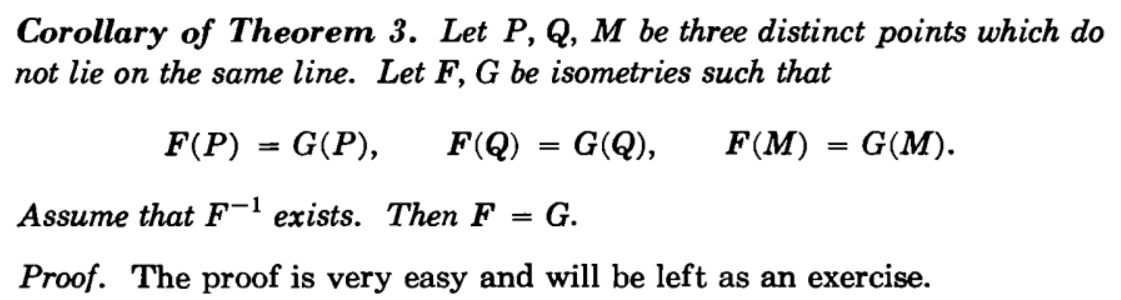
\includegraphics[width=0.6\textwidth]{images/coral.png}
\end{figure}

\begin{proof}
    Since $F(P) = G(P)$, $F(Q) = G(Q)$, and $F(M) = G(M)$
        it follows that $P = (F^{-1} \circ G)(P)$, $Q = (F^{-1} \circ G)(Q)$, and $M = (F^{-1} \circ G)(M)$.
    Now this is three fixed points so $F^{-1} \circ G$ is the identity mapping.
    Since $F^{-1} \circ G = I$ it follows that $G$ is the inverse of $F^{-1}$ which is $F$.
\end{proof}

\begin{tcolorbox}[title=Problem 6, breakable]
    Let $F \circ G \circ H$ be the composite of three isometries.
    Assume that $F^{-1}$, $G^{-1}$, $H^{-1}$ exist.
    Prove that $(F \circ G \circ H)^{-1}$ exists, and express this 
    inverse in terms of the inverses for $F, G, H$.
\end{tcolorbox}

\begin{proof}
    Let $P$ be an arbitrary point in the plane such that $(F \circ G \circ H)(P) = X$.
    Then 
    \begin{align*}
        &(F \circ G \circ H)(P) = X \\
        \iff& (H^{-1} \circ (F \circ G \circ H))(P) = H^{-1}(X) \\
        \iff& ((G^{-1} \circ H^{-1}) \circ (F \circ G \circ H))(P) = (G^{-1} \circ H^{-1})(X) \\
        \iff& ((F^{-1} \circ G^{-1} \circ H^{-1}) \circ (F \circ G \circ H))(P) = (F^{-1} \circ G^{-1} \circ H^{-1})(X) \\
        \iff& ((F \circ G \circ H)^{-1} \circ (F \circ G \circ H))(P) = (F^{-1} \circ G^{-1} \circ H^{-1})(X) \\
        \iff& I(P) = (F^{-1} \circ G^{-1} \circ H^{-1})(X) \\
        \iff& P = (F^{-1} \circ G^{-1} \circ H^{-1})(X)
    \end{align*}
    Therefore, $(F \circ G \circ H)^{-1} = H^{-1} \circ G^{-1} \circ F^{-1}$.
\end{proof}

\begin{tcolorbox}[title=Problem 7, breakable]
    Let $F$ be an isometry such that $F^7 = I$.
    Express $F^{-1}$ as a positive power $F$.
\end{tcolorbox}

\begin{proof}
Since $F^7 = I$, we have
\[
F^{-1} = I \circ F^{-1} = F^7 \circ F^{-1} = F^6.
\]
\end{proof}

\begin{tcolorbox}[title=Problem 8, breakable]
    Let $n$ be a positive integer and let $F$ be an isometry such that $F^n = I$.
    Express $F^{-1}$ as a positive power of $F$.
\end{tcolorbox}

\begin{proof}
    Since $F^n = I$, we have
\[
F^{-1} = I \circ I  \circ F^{-1} = F^n \circ F^n \circ F^{-1} = F^{2n - 1}.
\]
    Since $n \ge 1$ it follows that $2n \ge 2$ so $2n > 1$ and $2n - 1 > 0$.
\end{proof}

\begin{tcolorbox}[title=Problem 9, breakable]
    Consider the corners of a square centered at the origin.
    For convenience of notation, number these corners $1, 2, 3, 4$ as in Fig. $6-26$.

    Write the image of each one of these corners under the isometries.
    $H, V, H \circ V, V \circ H$. Just to show you an easy notation to 
    do this, we write down the images of these corners under rotation by 
    $90$\textdegree in the following form:

    \[
    \begin{bmatrix}
    1 & 2 & 3 & 4 \\
    2 & 3 & 4 & 1
    \end{bmatrix}
    \]

    This notation means that if $G$ is a rotation by $90$\textdegree,
    then $G(1) = 2$, $G(2) = 3$, $G(3) = 4$, and $G(4) = 1$.

    $H, V$ are the reflections along the horizontal line 
        and vertical line respectively.
\end{tcolorbox}

\begin{figure}[h]
    \centering
    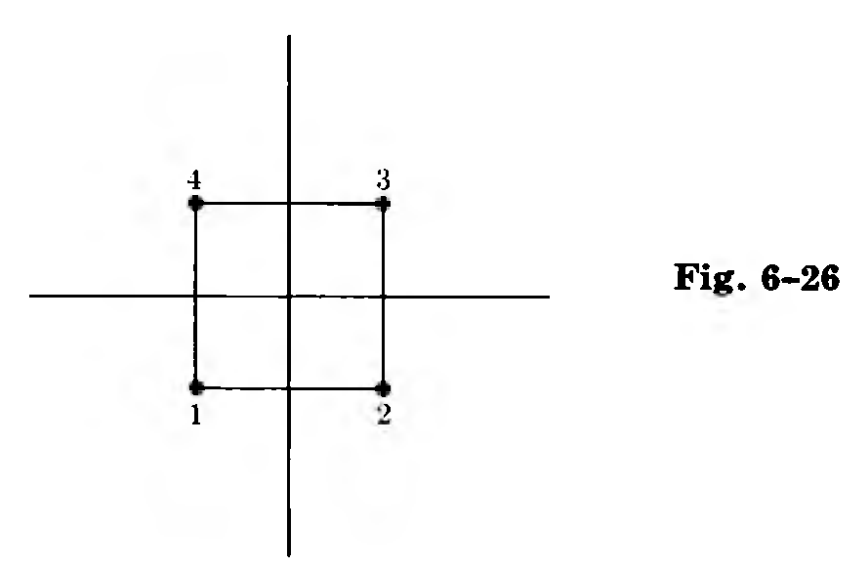
\includegraphics[width=0.6\textwidth]{images/square.png}
\end{figure}

\textbf{Solution:}

Image under $H$.
\[
\begin{bmatrix}
1 & 2 & 3 & 4 \\
4 & 3 & 2 & 1
\end{bmatrix}
\]
Image under $V$.
\[
\begin{bmatrix}
1 & 2 & 3 & 4 \\
2 & 1 & 4 & 3
\end{bmatrix}
\]
Image under $H \circ V$.
\[
\begin{bmatrix}
1 & 2 & 3 & 4 \\
3 & 4 & 1 & 2
\end{bmatrix}
\]
Image under $V \circ H$.
\[
\begin{bmatrix}
1 & 2 & 3 & 4 \\
3 & 4 & 1 & 2
\end{bmatrix}
\]

\begin{tcolorbox}[title=Problem 10, breakable]
    Let $G$ be a rotation by $90$\textdegree so that $G^4 = I$.
    Express $H \circ G \circ H$ as a power of $G$.
    For what positive integer $n$ do we have 
    \[H \circ G = G^n \circ H\]
    Write down the images of the corner of the square as in 
    the preceeding exercize, under the maps 
    $I, G, G^2, G^3, H, H \circ G, H \circ G^2, H \circ G^3, G \circ H, G^2 \circ H, G^3 \circ H$.
\end{tcolorbox}

\textbf{Solution:}

\[H \circ G \circ H = G^3\]
The following equation holds when $n = 3$.
\[H \circ G = G^n \circ H\]
% Identity
Image under $I$.
\[
\begin{bmatrix}
1 & 2 & 3 & 4 \\
1 & 2 & 3 & 4
\end{bmatrix}
\]

% Rotation by 90°
Image under $G$.
\[
\begin{bmatrix}
1 & 2 & 3 & 4 \\
2 & 3 & 4 & 1
\end{bmatrix}
\]

% Rotation by 180°
Image under $G^2$.
\[
\begin{bmatrix}
1 & 2 & 3 & 4 \\
3 & 4 & 1 & 2
\end{bmatrix}
\]

% Rotation by 270°
Image under $G^3$.
\[
\begin{bmatrix}
1 & 2 & 3 & 4 \\
4 & 1 & 2 & 3
\end{bmatrix}
\]

% Reflection H (horizontal)
Image under $H$.
\[
\begin{bmatrix}
1 & 2 & 3 & 4 \\
4 & 3 & 2 & 1
\end{bmatrix}
\]

% H followed by G
Image under $H \circ G$.
\[
\begin{bmatrix}
1 & 2 & 3 & 4 \\
1 & 4 & 3 & 2
\end{bmatrix}
\]

% H followed by G^2
Image under $H \circ G^2$.
\[
\begin{bmatrix}
1 & 2 & 3 & 4 \\
3 & 2 & 1 & 4
\end{bmatrix}
\]

% H followed by G^3
Image under $H \circ G^3$.
\[
\begin{bmatrix}
1 & 2 & 3 & 4 \\
2 & 1 & 4 & 3
\end{bmatrix}
\]

% G followed by H
Image under $G \circ H$.
\[
\begin{bmatrix}
1 & 2 & 3 & 4 \\
3 & 4 & 1 & 2
\end{bmatrix}
\]

% G^2 followed by H
Image under $G^2 \circ H$.
\[
\begin{bmatrix}
1 & 2 & 3 & 4 \\
2 & 1 & 4 & 3
\end{bmatrix}
\]

% G^3 followed by H
Image under $G^3 \circ H$.
\[
\begin{bmatrix}
1 & 2 & 3 & 4 \\
4 & 3 & 2 & 1
\end{bmatrix}
\]

\begin{tcolorbox}[title=Problem 13, breakable]
    Consider a triangle  whose three sides have equal length
    and whose three angles have the same measure, $60$\textdegree,
    as in Fig. $6-27$.

    The vertices of the triangle are numbered $1, 2, 3$.
    Let $G$ be a rotation by $120$\textdegree and let $V$,
    as usual, be reflection through the vertical axis.
    
    (a) Give the effect of the six isometries $I, G, G^2, V, VG, VG^2$
    on the vertices, using the same notation as exercize $9$.

    (b) Make up the multiplication table for these six isometries.
\end{tcolorbox}

\begin{figure}[h]
    \centering
    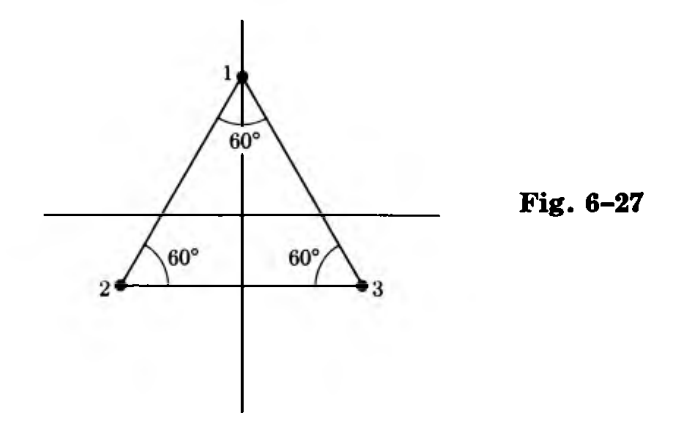
\includegraphics[width=0.6\textwidth]{images/triangle.png}
\end{figure}

\textbf{Solution:}

% Identity
Image under $I$.
\[
\begin{bmatrix}
1 & 2 & 3 \\
1 & 2 & 3
\end{bmatrix}
\]

% Rotation by 120°
Image under $G$.
\[
\begin{bmatrix}
1 & 2 & 3 \\
2 & 3 & 1 
\end{bmatrix}
\]

% Rotation by 240°
Image under $G^2$.
\[
\begin{bmatrix}
1 & 2 & 3 \\
3 & 1 & 2
\end{bmatrix}
\]

% Reflection by vertical
Image under $V$.
\[
\begin{bmatrix}
1 & 2 & 3  \\
1 & 3 & 2
\end{bmatrix}
\]

% Reflection by vertical and rotation by 120°
Image under $VG$.
\[
\begin{bmatrix}
1 & 2 & 3  \\
3 & 2 & 1
\end{bmatrix}
\]

% Reflection by vertical and rotation by 240°
Image under $VG^2$.
\[
\begin{bmatrix}
1 & 2 & 3  \\
2 & 1 & 3
\end{bmatrix}
\]

\[
\begin{array}{c|cccccc}
\circ & I & G & G^2 & V & VG & VG^2 \\ \hline
I & I & G & G^2 & V & VG & VG^2 \\
G & G & G^2 & I & VG^2 & V & VG \\
G^2 & G^2 & I & G & VG & VG^2 & V \\
V & V & VG & VG^2 & I & G^2 & G \\
VG & VG & VG^2 & V & G & I & G^2 \\
VG^2 & VG^2 & V & VG & G^2 & G & I
\end{array}
\]

\subsection{Characterization of Isometries}

\begin{tcolorbox}[title=Problem 1, breakable]
    Prove that every isometry has an inverse.
\end{tcolorbox}

\begin{proof}
    Let $F$ be an arbitrary isometry.
    There are four cases depending on the number of 
        fixed points under $F$.

    (\textbf{$\ge3$ fixed points}) By Theorem $3$, $F = I$
        which clearly has an inverse: $F^{-1} = I$.

    (\textbf{$2$ fixed points}) 
        Let $P$ and $Q$ be the two fixed points under $F$.
        By Theorem $4$, either $F$ is the identity, or $F$ is a reflection
        through the line $L_{PQ}$ passing through $P$ and $Q$.
        In the identity case, $F^{-1} = I$.
        If $F$ is a reflection, the inverse is also $F$: $F^{-1} = F$.

    (\textbf{$1$ fixed point}) 
        Let $P$ be the single fixed point under $F$.
        By Theorem $5$, either $F$ is a rotation about $P$, or 
        $F$ is a rotation composed with a reflection through a line through $P$.
        In the rotation case, $F^{-1}$ is the rotation by the opposite angle about $P$.
        In the rotation-reflection case, $F^{-1}$ is the reflection composed with the rotation by the opposite angle.

    (\textbf{no fixed points})
        By Theorem $6$, either $F$ is a translation,
            a composite of a translation and a rotation,
            or a composite of a translation, a rotation, and a reflection through a line.
        In the translation case, $F^{-1}$ is the translation by the opposite vector.
        In the translation-rotation case, $F^{-1}$ is the rotation by the opposite angle followed by translation by the opposite vector.
        In the translation-rotation-reflection case, $F^{-1}$ is the reflection followed by rotation by the opposite angle and translation by the opposite vector.

    Since these cases are exhaustive, every isometry has an inverse.
\end{proof}

\begin{tcolorbox}[title=Problem 2, breakable]
    If $P$ is a fixed point for an isometry $F$,
        prove that $P$ is also a fixed point 
        for $F^{-1}$.
\end{tcolorbox}

\begin{proof}
    Since $P$ is a fixed point under $F$ is follows that $F(P) = P$.
    By Problem $1$ we know that $F^{-1}$ exists.
    Applying $F^{-1}$ to both sides yields $P = F^{-1}(P)$.
    Therefore, $P$ is a fixed point of $F^{-1}$.
\end{proof}

\subsection{Congruences}

\begin{tcolorbox}[title=Problem 1, breakable]
    Prove that two discs of the same radius are congruent.
\end{tcolorbox}

\begin{proof}
    Let the first disc be $D(r, O)$, of radius $r$, centered at $O$, and let
    the other disc be $C(r, O')$, centered at $O'$. Let $T$ be the translation which
    maps $O$ on $O'$. We know that $T$ preserves distances. Hence if $P$ is at distance
    $\le r$ from $O$, then $T(P)$ is at distance $\le r$ from $T(O) = O'$. Hence the image of the
    disc $D(r, O)$ is contained in the circle $D(r, O')$. We must still show that every
    point on $D(r, O')$ is the image of a point on $D(r, O)$ under T. Let Q be a point
    at distance $\le r$ from $O'$. Note that the point
    \[P = T^{-1}(Q)\]
    is at distance $\le r$ from $O$, and that $T(P) = T(T^{-1}(Q)) = Q$.
\end{proof}

\begin{tcolorbox}[title=Problem 2, breakable]
    Let $S, S', S''$ be sets in the plane.
    Prove that if $S$ is congruent to $S'$,
        and $S'$ is congruent to $S''$,
        then $S$ is congruent to $S''$.
    Prove that if $S$ is congruent to $S'$,
        then $S'$ is congruent to $S$.
\end{tcolorbox}

\begin{proof}
    Suppose that $S$ is congruent to $S'$ and $S'$ is congruent to $S''$.
    Let $T$ be the isometry such that $T(S) = S'$.
    Let $F$ be the isometry such that $F(S') = S''$.
    Then $(F \circ T)(S) = F(T(S)) = F(S') = S''$.
    Note that a composition of isometries is an isometry.
    Thus $F \circ T$ is an isometry mapping $S$ to $S''$ 
        so $S$ is congruent to $S''$.
\end{proof}

\begin{proof}
    Suppose that $S$ is congruent to $S'$.
    Let $F$ be the isometry such that $F(S) = S'$.
    Since $F$ is an isometry it has an inverse $F^{-1}$.
    Then applying this to both sides yields $S = F^{-1}(S')$.
    Thus $S'$ is congruent to $S$.
\end{proof}

\begin{tcolorbox}[title=Problem 3, breakable]
    Prove that two squares whose sides have the 
        same length are congruent.
\end{tcolorbox}

\begin{proof}
    Let $S$ and $S'$ be two squares whose sides have the same length.
    Let $A, B, C, D$ be the vertices of $S$ in cyclic order.
    Let $O$ be the intersection of the diagonals $AC$ and $BD$.
    Since the diagonals of a square are equal in length and bisect each other
        at right angles, their intersection $O$ is equidistant from all vertices.
    Thus $O$ is the center of $S$.

    Similarly, let $A', B', C', D'$ be the vertices of $S'$ in cyclic order,
    and let $O'$ be the intersection of its diagonals (the center of $S'$).

    Let $T$ be the translation mapping $O$ to $O'$.
    Let $G$ be the rotation with respect to $O'$
        of $S'$ such that $(G \circ T)(A) = A'$.
    Because $G$ is a rotation about the center $O'$, it must also send 
        the point on the opposite end of that diagonal, namely $(G\circ T)(C)$, to $C'$, 
        and $(G\circ T)(D)$ to $D'$.
    If $(G \circ T)(B) \neq B'$, then perform  
        a reflection $R$ across the line connecting $(G \circ T)(A)$ and $(G \circ T)(C)$.
    Otherwise, let $R = I$ such that $I$ is the identity mapping.
    Let $F = R \circ G \circ T$.

    Thus $F(A) = A', F(B) = B', F(C) = C', F(D) = D'$, 
        and therefore $F(S) \subseteq S'$.
    Since $F$ is an isometry, it preserves distances and lines, so 
    every point of $S$ maps to points of $S'$ and vice versa, thus $F(S) = S'$.
\end{proof}

\newpage
\begin{tcolorbox}[title=Problem 4, breakable]
    Prove that any two lines are congruent.
\end{tcolorbox}


\begin{proof}
    Let $L$ and $L'$ be two lines. Pick points $P, Q \in L$ and $P', Q' \in L'$.  
    Using Section $6.4$ Problem $2$, since $d(P,Q) = d(P',Q')$, there exists an isometry $F$ such that $F(P) = P'$ and $F(Q) = Q'$.  

    Since $F$ preserves distances and maps two points on $L$ to two points on $L'$, it maps the entire line $L$ onto $L'$.  
    Therefore, the lines $L$ and $L'$ are congruent.
\end{proof}

\begin{tcolorbox}[title=Problem 5, breakable]
    Let $\triangle ABC$ be a triangle whose three angles all have $60$\textdegree.
    Prove that the sides have equal length.
    [Hint: From any vertex draw the perpendicular to the other side,
           and reflect through this perpendicular.]
\end{tcolorbox}

\begin{proof}
    Let $A, B, C$ be the vertices of a triangle whose three angles all have $60$\textdegree.
    Let $L$ be the perpendicular bisector of $\overline{AB}$, intersecting $\overline{AB}$ at its midpoint $O$.
    There are now two right triangles, namely $\triangle AOC$ and $\triangle BOC$,
        with right angles at $O$.
    These triangles share the side $\overline{OC}$.
    Since $L$ is the perpendicular bisector of $\overline{AB}$, we have $d(A, O) = d(B, O)$.
    Then
    \[
        d(A, C)^2 = d(A, O)^2 + d(O, C)^2 = d(B, O)^2 + d(O, C)^2 = d(B, C)^2.
    \]
    It follows that $d(A, C) = d(B, C)$.
    
    Apply similar steps but let $L$ be the perpendicular bisector of $\overline{BC}$,
        thus showing that $d(A, B) = d(A, C)$.

    Thus $d(A, B) = d(A, C) = d(B, C)$.
\end{proof}

\begin{proof}
    Let $A, B, C$ be the vertices of a triangle with all angles $60$\textdegree.
    Consider the perpendicular bisector $L$ of side $\overline{AB}$.
    Reflect the vertex $C$ across $L$ to a point $C'$. 

    Since the triangle has equal angles, this reflection maps the triangle to itself, so $C' = C$. 
    Reflection across the perpendicular bisector preserves distances, so
    \[
        AC = BC.
    \]
    Similarly, reflecting across the perpendicular bisector of $\overline{BC}$ gives
    \[
        AB = AC.
    \]
    Therefore, all three sides are equal:
    \[
        AB = BC = AC.
    \]
\end{proof}

\newpage
\begin{tcolorbox}[title=Problem 6, breakable]
    Prove Theorem $9$.
    At first you are not allowed to use Theorem $10$.
    If you were allowed to use Theorem $10$, how would 
        you deduce Theorem $9$ from it.

    \begin{theorem}
        Let $\triangle PQM$ and $\triangle P'Q'M'$ be right triangles 
            whose right anlges are at $Q$ and $Q'$ respectively.
        Assume that the corresponding legs have the same lengths,
            that is:
        \[d(P, Q) = d(P', Q')\]
        and 
        \[d(Q, M) = d(Q', M')\]
        Then the triangles are congruent.
    \end{theorem}
\end{tcolorbox}

\begin{proof}
    Let $T$ be the translation such that $T(Q) = Q'$.
    Let $G$ be the ration such that $(G \circ T)(P) = P'$.
    Finally, if $(G \circ T)(M) \not = M'$ apply a reflection on the line $\overline{P'Q'}$
    Let $F = G \circ T$.

    Thus, $G(Q) = Q'$, $G(P) = P'$, and $G(M) = M'$.

    Now let $O$ be any point on the segment $\overline{PQ}$.
    It follows that $d(P, Q) = d(F(P), F(Q)) = d(P, O) + d(Q, O) = d(F(P), F(O)) + d(F(Q), F(O))$.
    Then since $d(F(P), F(Q)) = d(F(P), F(O)) + d(F(Q), F(O))$, $F(O)$ lies on the segment $\overline{P'Q'}$.

    Now let $K$ be any point on the segment $\overline{P'Q'}$.
    Since $F$ is an isometry, it has an inverse; let $U = F^{-1}(K)$.
    Then $d(P, Q) = d(F^{-1}(P'), F^{-1}(Q')) = d(P, U) + d(U, Q)$ so $U$ lies on the segment $\overline{PQ}$.
    It follow that  $F(U) = F(F^{-1}(K)) = K$.

    Simlar arguments apply to $\overline{QM}$ and $\overline{PM}$.
    Thus the triangles are congruent.
\end{proof}

\begin{proof}
    Since the legs have the same length, by the Pythagorean Theorem their hypotenuses are of equal length.
    Thus the lengths of the sides of the triangles are equal.
    One can then easily apply Theorem $10$ to show the triangles are congruent.
\end{proof}

\begin{tcolorbox}[title=Problem 7, breakable]
    Let $\triangle PQM$ and $\triangle P'Q'M'$ be triangles 
        having one corresponding angle of the same measure,
        say $\angle PQM$ and $\angle P'Q'M'$ have the same measure,
        and having adjacent sides of the same length, i.e.
        \[d(P, Q) = d(P', Q') \text{ and } d(Q, M) = d(Q', M')\]
        Prove that the triangles are congruent.
\end{tcolorbox}

\begin{proof}
    Using Section $6.4$ Problem $2$, since $d(P,Q) = d(P',Q')$, 
        there exists an isometry $T$ such that $T(P) = P'$ and $T(Q) = Q'$.
    From the figure, if $T(M) \ne M'$ then perform a reflection $R$ through the line $\overline{P'Q'}$.
    Otherwise, let $R = I$ where $I$ is the identity mapping.
    Let $F = R \circ T$.

    If $R \ne I$, then reflecting about the line $\overline{P'Q'}$     
        ensures $F(M)$ points in the same direction as $M'$.
    Since $F$ is an isometry, it preserves distances, so $d(Q',F(M)) = d(Q,M) = d(Q',M')$.

    It follows that $F(P) = P', F(Q) = Q', F(M) = M'$.
    Thus the triangle's sides are the same length and applying Theorem $10$ shows 
        they are congruent.
\end{proof}


\begin{tcolorbox}[title=Problem 8, breakable]
    Prove that two rectangles having corresponding sides 
        of equal lengths are congruent.
\end{tcolorbox}

\begin{proof}
    Let $ABCD$ and $A'B'C'D'$ be the corners encountered cyclicly of two rectangles such that 
        $d(A,B) = d(A',B')$ and $d(B,C) = d(B',C')$.

    Let $T$ be the translation such that $T(A) = A'$.
    Let $G$ be the rotation about $A'$ such that $(G \circ T)(C)$ lies on the line through $A'$ and $C'$.
    If necessary, let $R$ be a reflection across the line $\overline{A'C'}$ to match $B$ and $B'$.
    Otherwise, let $R = I$ where $I$ is the identity mapping.
    
    % F should be the composition of those isometries.
    Thus $F = R \circ G \circ T$.

    Draw the diagonal $\overline{AC}$ in both rectangles. 
    This divides each rectangle into two right triangles: 
        $\triangle ABC$ and $\triangle ADC$ in the first rectangle, 
        and $\triangle A'B'C'$ and $\triangle A'D'C'$ in the second.

    Now let $O$ be any point on the segment $\overline{AC}$ of the first rectangle.
    It follows that $d(A,C) = d(A,O) + d(O,C) = d(A',F(O)) + d(F(O),C')$. 
    Then, by the Pythagorean Theorem, $F(O)$ lies on the segment $\overline{A'C'}$.

    Now let $K$ be any point on the segment $\overline{A'C'}$.  
    Since $F$ is an isometry, it has an inverse; let $U = F^{-1}(K)$.  
    Then $d(A,C) = d(F^{-1}(A'), F^{-1}(C')) = d(A,U) + d(U,C)$
        so $U$ lies on the segment $\overline{AC}$.  
    By definition of $U$, $F(U) = F(F^{-1}(K)) = K$.

    Hence the corresponding right triangles along the diagonals are congruent, 
        and therefore the rectangles $ABCD$ and $A'B'C'D'$ are congruent.
\end{proof}

\begin{tcolorbox}[title=Problem 9, breakable]
    Give a definition of the region bounded by a square in terms of line 
        segments. Same thing for a rectangle.
\end{tcolorbox}

\begin{definition}
    Let $S$ be a square with distinct parallel line segments $\overline{AB}$ and $\overline{CD}$.
    We can define the area of $S$ to be all points on all line segments formed by 
        points $X, Y$ where $X$ lies on $\overline{AB}$ and $Y$ lies on $\overline{CD}$.
    The area for a rectangle can be defined in precisely the same way
        with exception to letting $S$ be a rectangle.
\end{definition}

\begin{tcolorbox}[title=Problem 11, breakable]
    Let $\triangle PQM$ and $\triangle P'Q'M'$ be triangles whose corresponding
        angles have the same measures (i.e. the angle with vertex $P$ has the same 
        measure as the angle with vertex at $P'$, and similarly for the angles with
        vertices at $Q, Q'$ and $M, M'$). Assume that $d(P, Q) = d(P', Q')$.
    Prove that the triangles are congruent.
\end{tcolorbox}

\begin{proof}
    Using Section~$6.4$ Problem~$2$, since $d(P,Q) = d(P',Q')$, 
    there exists an isometry $T$ such that $T(P) = P'$ and $T(Q) = Q'$.
    From the figure, if $T(M) \ne M'$, then perform a reflection $R$ through the line $\overline{P'Q'}$.
    Otherwise, let $R = I$, where $I$ is the identity mapping.
    Let $F = R \circ T$.

    If $R \ne I$, then reflecting about the line $\overline{P'Q'}$
    ensures $F(M)$ lies on the same side of $\overline{P'Q'}$ as $M'$.
    Hence $F(P) = P'$ and $F(Q) = Q'$.
    Since corresponding angles are equal, the ray from $F(P)$ through $F(M)$
    coincides with the ray from $P'$ through $M'$, and the ray from $F(Q)$ through $F(M)$
    coincides with the ray from $Q'$ through $M'$.
    Therefore $F(M) = M'$, and $F$ maps all vertices of $\triangle PQM$
    to the corresponding vertices of $\triangle P'Q'M'$.

    Thus the triangles are congruent.
\end{proof}

\begin{tcolorbox}[title=Problem 12, breakable]
    Let $\triangle PQM$ be a triangle. 
    Let $L_1, L_2, L_3$ be the three lines which bisect 
        the three angles of the triangle, respectively.
    Let $O$ be the point of intersection of $L_1$ and $L_2$.
    Prove that $O$ lies on $L_3$.
    [Hint: From $O$, draw the perpendicular segments to the corresponding sides. 
     Prove that their lengths are equal.]
\end{tcolorbox}

\begin{figure}[h]
    \centering
    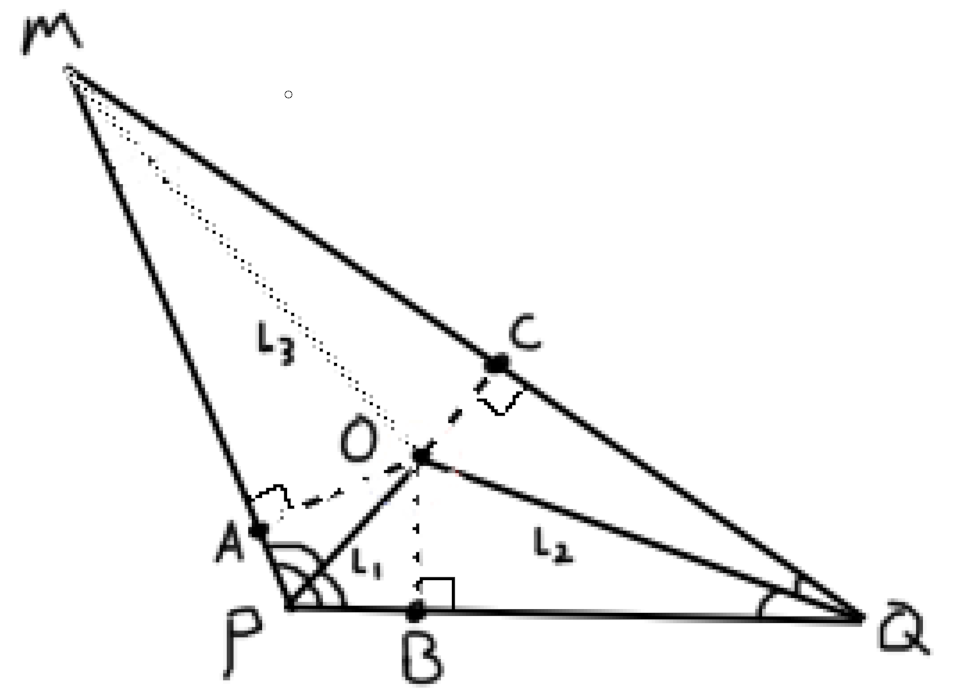
\includegraphics[width=0.6\textwidth]{images/last.png}
\end{figure}

\begin{proof}
    Let $A$, $B$, and $C$ be the feet of the perpendiculars from $O$ to the sides 
        $\overline{PM}$, $\overline{PQ}$, and $\overline{MQ}$ respectively.

    We first show that $\angle AOP$ and $\angle BOP$
        are equivalent.
    The sum of the angles of $\triangle AOP$ and $\triangle BOP$ can 
        be expressed as $90 + \angle APO + \angle AOP$
        and $90 + \angle BPO + \angle BOP$, respectively.
    These sums must both equal $180$, so
        \[
            90 + \angle APO + \angle AOP = 90 + \angle BPO + \angle BOP.
        \]
    But $\angle APO = \angle BPO$, since $L_1$ bisects $\angle P$.
    Therefore, $\angle AOP = \angle BOP$.

    Thus  $\triangle AOP$ is a reflection of $\triangle BOP$ across $L_1$.
    Therefore their corresponding sides are equal,
        so the perpendicular distances from $O$ to $\overline{PM}$ and $\overline{PQ}$ are equal,
        and thus $OA = OB$.

    By the same reasoning, since $O$ also lies on $L_2$, which bisects $\angle Q$,
    the right triangles $\triangle OBQ$ and $\triangle OCQ$ are reflections across $L_2$,
    giving $OB = OC$.

    Therefore $OA = OB = OC$.
    A point equidistant from all three sides of a triangle lies on the bisector of the remaining angle.
    Hence, $O$ lies on $L_3$.
\end{proof}